\chapter{Background}
this is short and needs a lot more detail and also figures.

This section briefly reviews the current techniques for lung perfusion and hemodynamic
monitoring, and provides a general overview 
of the state of 3D EIT as used for thoracic imaging and monitoring.

\section{Electrical Impedance Tomography}

\subsection{Impedance Imaging}
Impedance imaging has been in use since the early 1900s for geophisical applications.  
Originally introduced as a technique to image below the earth’s surface, 
current was transmitted between two electrodes placed into the ground and any 
anomalies in subsurface conductivity produced deviation 
in the equipotential lines. 
Including current injections and measurements from multiple locations and using known 
electrical properties of geological structures Conrad Schlumberger identified
features of underground geological structures~\parencite{allaud_schlumberger_1977}.

These same techniques can be applied in biomedical applications where
voltage is measured on an array of body surface electrodes 
while current is applied between select electrode pairs(\fref{fig:cur_equip_line}). 
Due to impedance differences associated with biological tissues and their physiological 
function~\parencite{Geddes1967,McAdams1995}
EIT has been proposed for a wide range of applications from thoracic monitoring to neuronal and 
brain imaging~\parencite{Holder1992,Frerichs2016}. 

\begin{figure}
   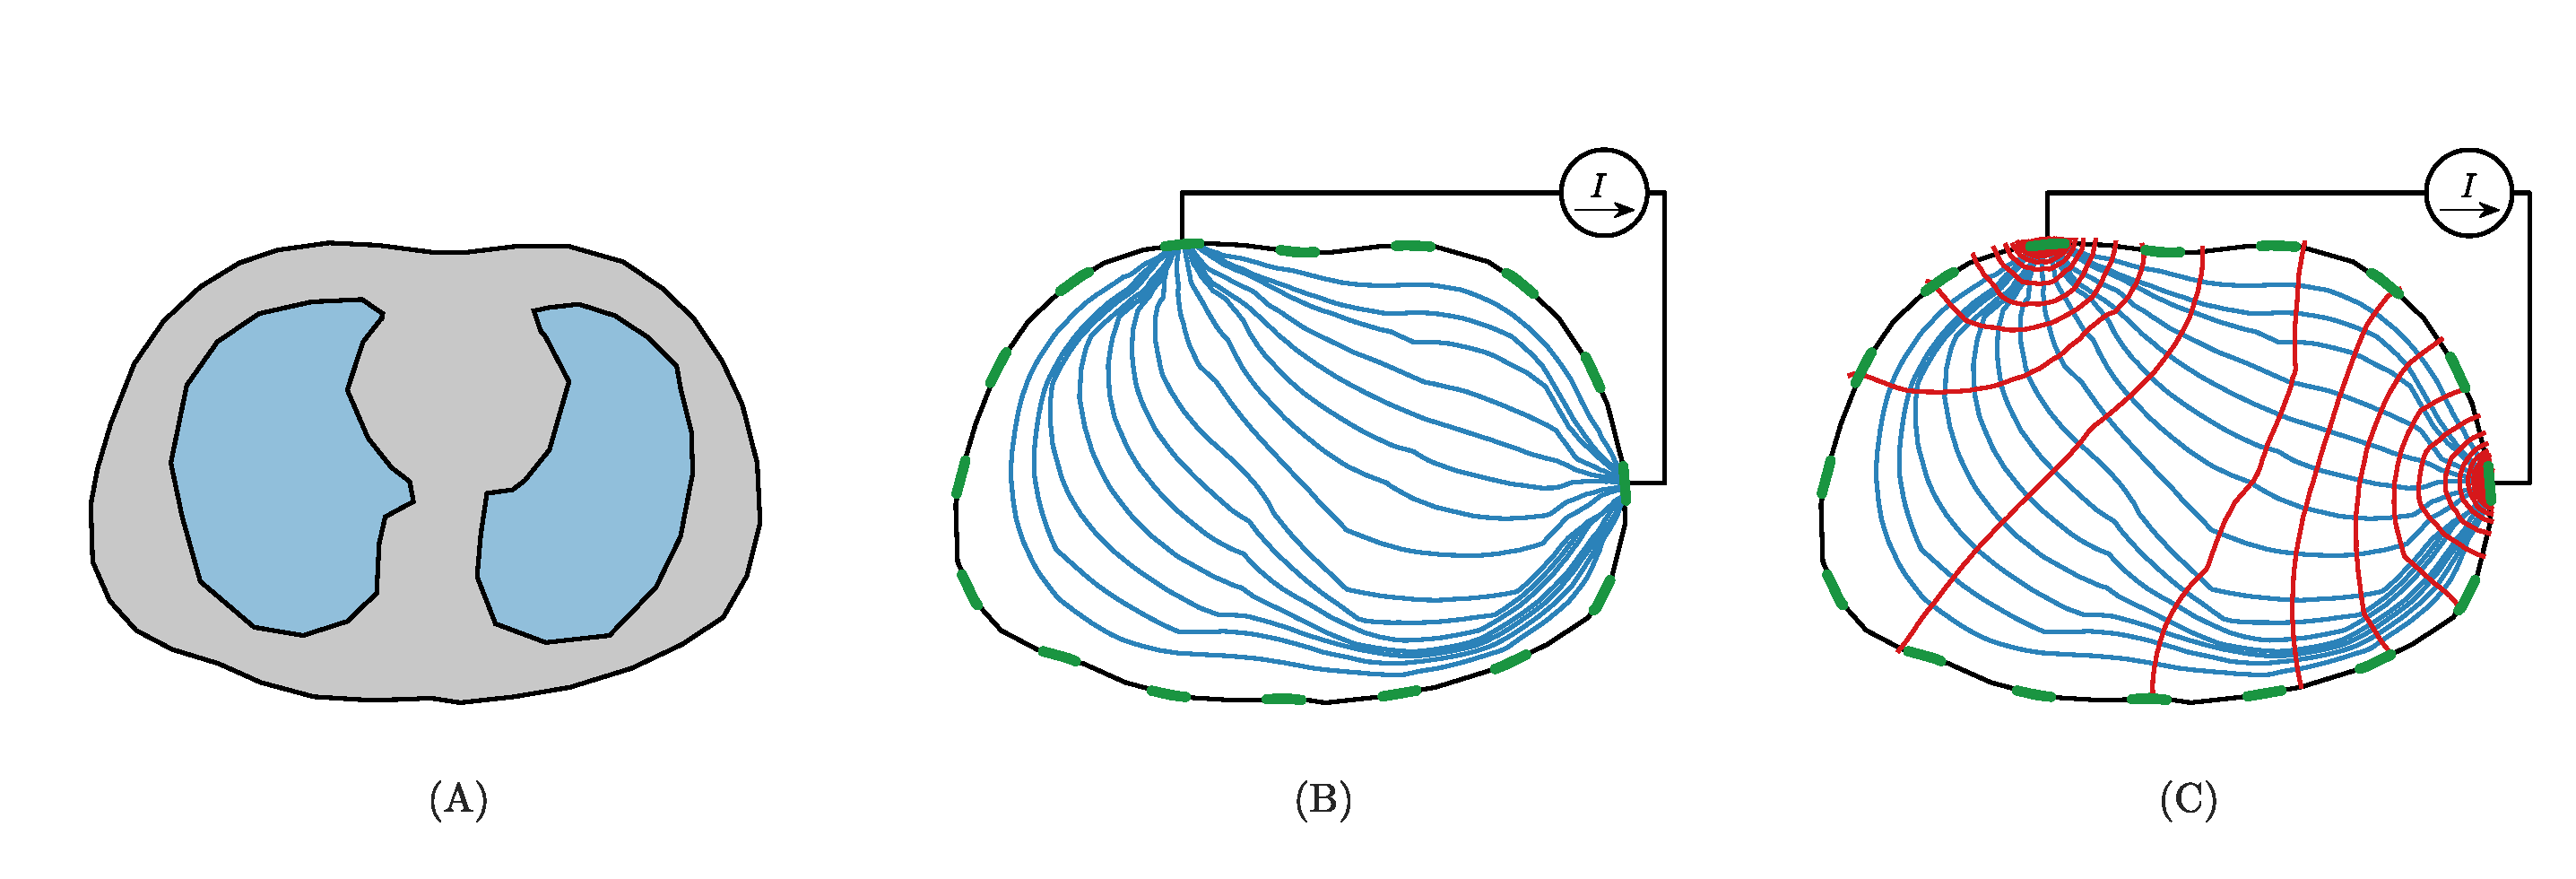
\includegraphics[width=\textwidth]{chapter2-background/imgs/current_and_equipotential_lines.pdf}
   \caption[Current and Equipotential lines]{\label{fig:cur_equip_line} 
   (A) A body comprising tissues of different conductivity, (B) Electrodes are placed on the surface 
   and current is injected between a pair or electrodes. The current pathways are indicated 
   by the blue lines. (C) The resulting equipotential lines within the body.}
\end{figure}

\subsection{Bioimpedance}


\TODO{
    Discuss high and low frequencies and the impednace of the tissues of interest  \\
    What constrasts are easy and which are interesting?
    }

\subsection{Forward Problem}
Using the quasi-static 
formulations of Maxwell's equations, the potential distribution $u$ can be used 
compute the conductivity $\rho$ and generate images.

\subsection{Discretization and the Finite Element Method}

\subsection{Image Reconstruction}

\subsubsection{2D reconstruction}

\subsubsection{3D Reconstruction}
The majority of EIT measurements are done with a single ring of external electrodes but 
in practice, electrical current cannot  be confined to a single plane
and using a two dimensional electrode configuration can significantly
impact the capabilities of \acrshort{eit}~\parencite{Rabbani1991}.
The use of 3D electrode configurations in \acrshort{eit}
was introduced in 1996~\parencite{Metherall1996} to overcome the 
inherent limitations of 2D measurements, but it is still not widely used today.
It is thought this is due to the increased complexity of 3D images
and the subsequent analysis~\parencite{Grychtol2019}.

It has been shown that externally placed 3D electrode configurations
consisting of two electrode planes
can improve the sensitivity distribution and image quality~\parencite{Grychtol2016},
but there is still limited sensitivity in the central-most regions 
of the chest.
The concept of using internal esophageal electrodes has been presented
previously~\parencite{Pilkington1989,Schuessler1995}
as a method to improve internal sensitivity 
and reconstruction quality,
but has not been widely used or simulated.
Several studies have shown that there may be several advantages to using an internal
electrode in \acrshort{eit} recordings; 
Measurements with an internal electrode have been 
shown to reconstruct images equally as well as configurations with 
twice as many external electrodes~\parencite{Schuessler1995},
and have shown an increase in sensitivity in a central region 
of interest~\parencite{Kwon2013,Czaplik2014,Farooq2014}.
\subsubsection{GREIT}
\subsubsection{Image Regularization}

\subsection{Internal Electrodes}
\subsubsection{Internal Reference Electrodes}
\subsubsection{Inverse Source localization (time permitting)}


\subsection{Imaging Techniques}

\TODO{
    Time Difference \\
    Frequency Difference \\
    Absolute \\ 
}

\subsubsection{Absolute}

Imaging the absolute difference in tissue impedance is challenging due to the non-linear trajectory of 
electrical current, individual anatomy and difference in electrode contact impedance. 

\subsubsection{Frequency Difference}

\subsubsection{Time Difference}
Time difference EIT uses a reference frame to image the change in conductivity between 
two points in time and allows for imaging of functional activity such as the inflation of the lungs 
and the flow of blood.






% TODO in the thesis go into absolute imaging vs time difference imaging in depth here!!!

\section{Lung perfusion monitoring}
\subsection{Sensitivity to Blood Movement}
\subsection{Contrast agent injection}
\subsection{Frequency Filtering}


Monitoring lung ventilation is one of the most
established clinical uses of 
\acrshort{eit}, presented initially by Barber and Brown~\parencite{Barber1984}.
EIT has also been used as a tool to monitor blood 
perfusion~\parencite{Brown1992} and hemodynamic parameters such as 
cardiac output~\parencite{Braun2018} and blood pressure~\parencite{Sola2011,Proenca2017}. 
While the spatial resolution of \acrshort{eit} is much lower than 
intermittent imaging techniques such as \acrfull{ct} or \acrfull{mri},
\acrshort{eit} can have a high temporal resolution enabling continuous or frequent 
monitoring without concerns regarding radiation exposure.
This thesis focuses on time difference EIT for thoracic hemodynamic imaging and monitoring applications. 

EIT is sensitive to the movement of blood in two main ways. First, a conductivity-contrasting 
bolus solution injected into a vein or artery can be used to image the transit of blood through the body
and second, the pulsatile changes in conductivity at the cardiac frequency can be isolated 
through digital filtering~\parencite{Leathard1994}.
This document proposes methods and techniques to identify and isolate these impedance variations
to monitor lung perfusion and 
aortic flow.

A perfusion scan is a technique for imaging the blood flow through the lungs
and when compared with ventilation images can be used to detect pulmonary embolisms
when a mismatch is identified. Clinically pulmonary perfusion is done using 
lung nuclear medical imaging such as \acrfull{spect}~\parencite{Parker2012}. Radio-isotopes are inhaled through a mask 
for ventilation imaging and injected into the blood to image pulmonary perfusion. 
Images taken on a gamma camera are compared to look for a mismatch between the ventilation
and perfusion distribution. This method of 
measuring lung perfusion is slow and exposes the subject to low-dose radiation.

EIT has been evaluated for its ability to measure cardiac output and
lung perfusion since the late 1980s~\parencite{Eyuboglu1989,Blottt1992,Brown1992,Frerichs2002}. 
Since then, various configurations of EIT have been evaluated~\parencite{Borges2012,Nguyen2015}.
Due to the speed and safety of measurement acquisition, EIT might be used to continuously monitor 
perfusion in subjects.

There are two main challenges with perfusion monitoring using EIT. First, impedance change due to ventilation 
is 10 times larger than the impedance change due to cardiac-frequency pulsatile activity~\parencite{Deibele2008}
and second, the pulsatile activity outside the lung region can overwhelm the lung perfusion signal~\parencite{Stowe2019}. 
There are several techniques available to mitigate the difference 
in magnitude such as: pausing ventilation; administering a 
conductivity-contrasting bolus through the heart and lungs via the jugular~\parencite{Frerichs2002};
and digital filtering to isolate activity at the cardiac frequency~\parencite{Leathard1994}. 

When breathing is paused, the signals based only on the cardiac activity can be more easily extracted. 
It was found that during apnoea the global impedance recorded with EIT measurements corresponded with stroke volume 
measured using the 
thermodilution method with a pulmonary arterial catheter~\parencite{Fagerberg2009}.
Ventilation perfusion ratios have been calculated during apnoea by comparing 
ventilation and perfusion signal amplitude with a specified region of 
interest~\parencite{Fagerberg2009a}.
There is some concern that the perfusion measured during apnoea may not accurately represent 
true perfusion during regular respiration as the apnoea impacts the regular respiratory cycle~\parencite{Leonhardt2012}.

Using the conductivity-contrasting bolus injection EIT perfusion imaging has been compared to 
SPECT measurements, and blood flow has been imaged from the right heart into the lungs and back into the left heart
using 5-10\% hypertonic saline~\parencite{Frerichs2002,Borges2012}. This technique is promising 
for imaging lung perfusion, but is slow and requires the placement of a venous catheter 
and repeated saline injections to obtain perfusion measures. 

The final method to calculate perfusion using EIT is through filtering to isolate the 
cardiac related signal. Previous work has shown that principal component analysis (PCA) 
can be used to separate ventilation and cardiac frequency signals and identify the component 
related to the heart~\parencite{Deibele2008}. Once the cardiac-frequency component of the 
EIT signal is identified the pulmonary component must also be isolated. Other than visual 
identification of the lung region or manually selecting a region of interest,
there are few good solutions for isolating pulsatile activity within the lung region.

The use of 3D configurations to differentiation between pulsatile activity 
in the heart and lungs could allow for an improved perfusion measure 
using EIT, and a means of continuously monitoring perfusion during ventilation.

\section{Aortic flow monitoring}

Continuous bedside monitoring appears to be one of the most
promising future applications of \acrshort{eit} due to the high 
temporal resolution, and concerns with other imaging modalities 
and the associated radiation 
exposure. 

%There are several hemodynamic parameters that are widely used to asses cardiovascular 
%health. One of the most used is cardiac output (CO), the amount of blood pumped through the
%heart in one minute.
%The two most used method is
%thermodilution using a Swan-Ganz catheter~\parencite{Khalil1963} in the pulmonary artery, 
%which determines CO by injecting a solution with a known temperature and 
%measuring the temperature change~\parencite{ReuterDaniel2010}. This method is considered the gold standard of 
%CO monitoring~\parencite{Joosten2017}.

Another potential use of EIT is to replace invasive monitoring techniques
such as catheterized measurements of pulmonary arterial pressure.
Recent studies have evaluated EIT as a method of determining 
pulmonary arterial pressure using pulse wave velocity in the 
descending aorta in 2D~\parencite{Braun2018a,Proenca2017,Proenca2016}.
EIT was a used in conjunction with ECG signals and shown to have a high correlation
with pulmonary arterial pressure values from from Doppler echocardiography~\parencite{Proenca2016}.

An analysis of hemodynamic measures using EIT found that measures of stroke 
volume and pulmonary arterial pressure are sensitive to electrode placement and
interference from pulmonary signals~\parencite{Braun2018a}. 
The solution proposed in this document uses an arrangement of internal electrodes placed in the 
esophagus adjacent to the aorta to increase the sensitivity to changes and improve detection 
accuracy and elimination of pulmonary signals.

Improving tracking and imaging of the aorta is also important because it
has additional clinical uses: it  can be used as a physiological landmark to identify
the back of the lungs, and can be used to continuously monitor blood pressure by
calculating the pulse transit time. 



\acrshort{eit} has been used clinically to monitor lung perfusion 
in an animal model~\parencite{Leonhardt2012,Nguyen2012}, and it is theorized that 
the use of an internal electrode for increased sensitivity may allow for 
imaging of blood flow in the aorta. 
There is great interest in monitoring cardiac parameters
using \acrshort{eit} to determine \acrfull{sv}~\parencite{Proenca2017,Braun2018}, and increased
sensitivity close to the heart also has the potential to improve
these measures.

While there have been some studies researching electrode placement for cardiac
imaging in 2D~\parencite{Noordegraaf1996} and 
3D electrode configurations~\parencite{Graham2007}, there has 
been little research into determining the optimal 3D external electrode configurations
for imaging the heart and aorta. 

Additionally when using alternate electrode configurations the current injection and 
measurement patterns must also be investigated. It has been suggested that  an internal electrode
in 2D
should not be used for current injection in asymmetrical models
as the reconstruction performance deteriorates~\parencite{NasehiTehrani2012}. 
It is unclear 
to what degree injection patterns affect the resulting sensitivity when
internal electrodes and alternate electrode arrangements are used in 3D.

This work aims to investigate internal and 
external electrode configurations for use in imaging blood movement 
in the thorax, and develop techniques to extract measures of 
aortic flow and lung perfusion from these reconstructions.

%\subsubsection{3D \acrshort{eit} image reconstruction}
%It has been shown that when the continuous boundary voltages of a surface are
%known, there is a unique solution to the inverse problem used to calculate internal 
%conductivity~\parencite{Calderon2006},
%but EIT uses discrete measurements of boundary voltage 
%and there is no unique solution. 
%
%In order to reconstruct EIT images prior information and smoothing 
%must be used to obtain a solution. There are several reconstruction methods used in 
%EIT including Tikhonov regularization~\parencite{Tikhonov1977} and 
%standardized methods for EIT such as GREIT~\parencite{Adler2009}.
%A version of GREIT for 3D reconstructions~\parencite{Grychtol2016}
%is used in this work.
